\chapter{उत्परिवर्तन और जीनोम की विविधता}\label{ch:b2:genome-diversification}

किसी प्रतिजैविक से सनी प्लेट पर एक अरब जीवाणु फैलाइए और अगली सुबह
मुट्ठी भर निवह उग आए मिलेंगे। क्या उस औषधि ने उन कोशिकाओं को उसका
प्रतिरोध करना सिखाया, या वे उससे मिलने से पहले ही प्रतिरोधी थीं? यह
प्रश्न दार्शनिक लगता है और 1943 में बड़ी सुंदरता के एक प्रयोग से सुलझा
लिया गया: प्रतिरोधी कोशिकाएँ पहले से वहीं थीं, और वे ऐसे \omterm{def:b2:genome-diversification:mutation}{उत्परिवर्तनों} से
बनी थीं जो यादृच्छिक रूप से हुए, अपनी उपयोगिता की परवाह किए बिना। यह
अध्याय उसी विविधता के स्रोतों के बारे में है --- नक़ल की त्रुटियाँ,
रासायनिक दुर्घटनाएँ, कूदते जीन, कोशिकाओं के बीच अदला-बदली किए जाते जीन,
जीनों और पूरे जीनोमों का द्विगुणन --- और इस बारे में कि वे कितनी तेज़
चलते हैं। वरण, जो इस विविधता को छाँटता है,
\cref{ch:b2:population-genetics} का विषय है; यहाँ विषय यह है कि कच्चा
माल कहाँ से आता है।

\section{उत्परिवर्तन}

\begin{definition}[उत्परिवर्तन और उसके प्रकार]\label{def:b2:genome-diversification:mutation}
\index{उत्परिवर्तन}\index{बिंदु उत्परिवर्तन}\index{चौखटा-विस्थापन}\index{गुणसूत्रीय पुनर्विन्यास}
\emph{उत्परिवर्तन} जीनोम के अनुक्रम में हुआ ऐसा परिवर्तन है जो
वंशागत होता है। \emph{बिंदु उत्परिवर्तन} एक या कुछ क्षारक बदलते हैं:
\emph{प्रतिस्थापन} एक क्षारक की जगह दूसरा रख देता है (\emph{संक्रमण}
प्यूरीन की जगह प्यूरीन या पिरिमिडीन की जगह पिरिमिडीन रखता है,
A$\leftrightarrow$G या C$\leftrightarrow$T; \emph{पर्यावर्तन} वर्ग ही
बदल देता है); \emph{अंतर्वेशन} या \emph{विलोपन} क्षारक जोड़ता या हटाता
है। किसी कूटलेखी अनुक्रम में कोई प्रतिस्थापन \emph{मूक} है यदि नया
कोडॉन वही ऐमीनो अम्ल बताए, \emph{कुअर्थी} यदि वह कोई दूसरा बताए,
\emph{निरर्थक} यदि वह कोई विराम बना दे; और तीन के गुणज से भिन्न कोई
अंतर्वेशन या विलोपन वाचन-चौखटा खिसका देता है (\emph{चौखटा-विस्थापन})
और आगे का हर कोडॉन गड़बड़ा देता है। \emph{गुणसूत्रीय पुनर्विन्यास} बड़े
खंड हिलाते हैं: विलोपन, द्विगुणन, प्रतिलोमन, गुणसूत्रों के बीच
स्थानांतरण। \emph{जीनोम उत्परिवर्तन} गुणसूत्रों की संख्या बदलते हैं:
\emph{असुगुणिता} (एक गुणसूत्र अधिक या कम, जैसे त्रिसूत्रता 21) और
\emph{\omterm{def:b2:genome-diversification:polyploidy}{बहुगुणिता}} (पूरे अतिरिक्त समुच्चय)। किसी कायिक
कोशिका का उत्परिवर्तन केवल उसी कोशिका की संतति को मिलता है; जनन वंशक्रम
का उत्परिवर्तन जीव की संतति को मिलता है, और विकास के लिए केवल यही मायने
रखते हैं।
\end{definition}

\begin{omfigure}
\begin{tikzpicture}[every node/.style={font=\small\ttfamily}]
  \node[anchor=west] at (0,2.4) {ATG GAA TTC CTG AAG TGG TAA};
  \node[anchor=west, font=\scriptsize\rmfamily] at (5.6,2.4) {Met Glu Phe Leu Lys Trp विराम --- वन्य प्ररूप};
  \node[anchor=west] at (0,1.7) {ATG GA\textcolor{omThm}{G} TTC CTG AAG TGG TAA};
  \node[anchor=west, font=\scriptsize\rmfamily] at (5.6,1.7) {Met Glu Phe Leu Lys Trp विराम --- मूक};
  \node[anchor=west] at (0,1.0) {ATG G\textcolor{omThm}{T}A TTC CTG AAG TGG TAA};
  \node[anchor=west, font=\scriptsize\rmfamily] at (5.6,1.0) {Met \textcolor{omThm}{Val} Phe Leu Lys Trp विराम --- कुअर्थी};
  \node[anchor=west] at (0,0.3) {ATG \textcolor{omThm}{T}AA TTC CTG AAG TGG TAA};
  \node[anchor=west, font=\scriptsize\rmfamily] at (5.6,0.3) {Met \textcolor{omThm}{विराम} --- निरर्थक};
  \node[anchor=west] at (0,-0.4) {ATG GA\textcolor{omThm}{C}A TTC CTG AAG TGG TAA};
  \node[anchor=west, font=\scriptsize\rmfamily] at (5.6,-0.4) {Met \textcolor{omThm}{Asp Ile Pro Glu Val} \dots{} --- चौखटा-विस्थापन};
\end{tikzpicture}

{\small किसी छोटे कूटलेखी अनुक्रम में \omterm{def:b2:genome-diversification:mutation}{बिंदु उत्परिवर्तन} (परिवर्तन लाल में)।
कोई मूक प्रतिस्थापन प्रोटीन वैसा ही छोड़ देता है; कोई कुअर्थी एक अवशेष
बदल देता है; कोई निरर्थक उसे काट देता है; और एक ही अंतर्वेशित क्षारक
चौखटा खिसका देता है और आगे का सब कुछ फिर से लिख देता है।}
\end{omfigure}

\begin{proposition}[उत्परिवर्तन कहाँ से आते हैं]\label{prop:b2:genome-diversification:sources}
\index{उत्परिवर्तजन}\index{विऐमीनन}\index{विप्यूरीनन}
तीन स्रोत। \emph{प्रतिकृतिकरण की त्रुटियाँ}: DNA पॉलिमरेज़ लगभग
$10^{5}$ में एक बार कोई क्षारक ग़लत जगह रख देता है; उसका प्रूफ़-पठन
एक्सोन्यूक्लिएज़ अधिकांश हटा देता है और $10^{7}$ में एक छोड़ता है; और
बेमेल-मरम्मत, जो प्रतिकृतिकरण द्विशाख के पीछे चलती है और नए रज्जु को
पुराने के विरुद्ध सुधारती है, अंतिम त्रुटि दर को प्रति क्षारक प्रति
प्रतिकृतिकरण लगभग $10^{-9}$ से $10^{-10}$ तक ले आती है।
\emph{स्वतःस्फूर्त रसायन}: हर मानव कोशिका में रोज़ कोई \num{10000}
प्यूरीन अपनी शर्कराओं से झड़ जाते हैं (\emph{विप्यूरीनन}) और सौ
साइटोसीन एक ऐमीनो समूह खो देते हैं (\emph{विऐमीनन}, जो C को U बना देता
है, और वह A से युग्मित होता है); दोनों की मरम्मत होती है, पर सदा नहीं।
\emph{उत्परिवर्तजन}: पराबैंगनी प्रकाश पड़ोसी थाइमीनों को वेल्ड करके
द्विलक बना देता है; आयनकारी विकिरण रज्जु तोड़ देता है; ऐल्किलनकारी कारक
और नाइट्रस अम्ल क्षारक बदल देते हैं; अंतर्वेशी रंजक क्षारक युग्मों के
बीच सरक जाते हैं और \omterm{def:b2:genome-diversification:mutation}{चौखटा-विस्थापन} कराते हैं; श्वसन के ऑक्सीजन मूलक
ग्वानीन को ऑक्सीकृत कर देते हैं। प्रति क्षारक दर नन्ही है; जीनोम के
आकार और कोशिकाओं की संख्या से गुणा कर दें तो नहीं।
\end{proposition}

\begin{theorem}[प्रति जीनोम और प्रति आबादी उत्परिवर्तन]\label{thm:b2:genome-diversification:rate}
\index{उत्परिवर्तन दर}
यदि \omterm{thm:b2:genome-diversification:rate}{उत्परिवर्तन दर} प्रति क्षारक युग्म प्रति प्रतिकृतिकरण $u$ हो और
जीनोम में $G$ क्षारक युग्म हों, तो हर प्रतिकृतिकरण औसतन
$U = uG$ नए \omterm{def:b2:genome-diversification:mutation}{उत्परिवर्तन} बनाता है, और $N$ कोशिकाओं की कोई आबादी प्रति
पीढ़ी $UN$। \emph{E.~coli} के लिए ($u \approx \qty{5e-10}{}$, $G =
\qty{4.6e6}{}$): $U \approx 0.002$, यानी पाँच सौ में एक कोशिका कोई नया
\omterm{def:b2:genome-diversification:mutation}{उत्परिवर्तन} ढोती है --- पर $10^{9}$ कोशिकाओं का संवर्धन प्रति पीढ़ी
बीस लाख बनाता है, और $3G \approx 1.4\times
10^{7}$ संभव एक-क्षारक परिवर्तनों में से हर एक उसमें हर कुछ पीढ़ियों
में कहीं न कहीं उठ खड़ा होता है। किसी मनुष्य के लिए ($u \approx \qty{1.2e-8}{}$ प्रति
पीढ़ी, अगुणित समुच्चय में $G = \qty{3.2e9}{}$, दो समुच्चय): हर
बच्चा लगभग \num{75} नए \omterm{def:b2:genome-diversification:mutation}{उत्परिवर्तन} ढोता है, जिनमें एक या दो
कूटलेखी अनुक्रम में होते हैं।
\end{theorem}
\begin{proof}
हर क्षारक स्वतंत्र रूप से नक़ल होता है और उसमें त्रुटि की प्रायिकता $u$
है, इसलिए प्रति जीनोम-प्रति में त्रुटियों की संख्या $G$ स्वतंत्र विरल
घटनाओं का योग है, जिसका माध्य $uG$ है (और जो लगभग पॉइसों वितरित है)।
$N$ कोशिकाएँ $N$ प्रतियाँ बनाती हैं। मानव आँकड़ा द्विगुणित जीनोम के लिए
$u$ को $2G$ से गुणा करता है; और प्रति पीढ़ी दर प्रति पीढ़ी ही है, प्रति
प्रतिकृतिकरण नहीं, क्योंकि जनन कोशिकाएँ निषेचन और अगले निषेचन के बीच
अनेक प्रतिकृतिकरण से गुज़रती हैं।
\end{proof}

\begin{theorem}[किसी बढ़ते संवर्धन में उत्परिवर्ती]\label{thm:b2:genome-diversification:luria}
\index{लूरिया--डेलब्रुक प्रयोग}\index{उच्चावचन परीक्षण}
$N_0$ से $N$ कोशिकाओं तक बढ़ा कोई संवर्धन, जिसमें कोई दिया हुआ \omterm{def:b2:genome-diversification:mutation}{उत्परिवर्तन}
हर कोशिका-विभाजन पर $m$ प्रायिकता से होता है, अंत में \omterm{def:b2:genome-diversification:mutation}{उत्परिवर्तन}
\emph{घटनाओं} की माध्य संख्या $m(N - N_0)$ रखता है, और उत्परिवर्ती
\emph{कोशिकाओं} की माध्य संख्या
\[
\langle M\rangle = m\,N\,\ln\frac{N}{N_0},
\]
जो घटनाओं की संख्या से बड़ी है, क्योंकि कोई जल्दी हुआ \omterm{def:b2:genome-diversification:mutation}{उत्परिवर्तन} एक
क्लोन बसा देता है। उत्परिवर्ती कोशिकाओं की संख्या एक संवर्धन से दूसरे
संवर्धन में ज़बरदस्त रूप से बदलती है (विरल आरंभिक घटनाएँ ``जैकपॉट'' देती
हैं), जबकि यदि \omterm{def:b2:genome-diversification:mutation}{उत्परिवर्तन} प्लेट पर बोते समय प्रेरित होते, तो वह ऐसे
पॉइसों नियम का पालन करती जिसका प्रसरण उसके माध्य के बराबर होता। जिन
संवर्धनों में एक भी उत्परिवर्ती नहीं, उनका अंश $p_0 = e^{-m(N - N_0)}$ है, जिससे $m$ सीधे मिल जाता है।
\end{theorem}
\begin{proof}
$n$ से $n + \mathrm{d}n$ कोशिकाओं तक की वृद्धि में $\mathrm{d}n$
विभाजन लगते हैं, और हर एक \omterm{def:b2:genome-diversification:mutation}{उत्परिवर्तन} का एक अवसर है, इसलिए उस अंतराल
में $m\,\mathrm{d}n$ घटनाएँ होती हैं; जोड़ने पर कुल $m(N - N_0)$ घटनाएँ।
जब संवर्धन में $n$ कोशिकाएँ हों तब हुआ कोई \omterm{def:b2:genome-diversification:mutation}{उत्परिवर्तन} ऐसा क्लोन बसाता
है जो संवर्धन के साथ क़दम मिलाकर बढ़ता है और अंत में $N/n$ कोशिकाओं का
होता है; इसलिए उत्परिवर्ती कोशिकाओं की प्रत्याशित संख्या
$\int_{N_0}^{N} m\,(N/n)\,\mathrm{d}n = mN\ln(N/N_0)$ है। घटनाएँ विरल
और स्वतंत्र हैं, इसलिए उनकी संख्या $m(N - N_0)$ माध्य की पॉइसों है, और
एक भी न होने की प्रायिकता $e^{-m(N - N_0)}$ है।
\end{proof}
\begin{proof}[प्रमाण-सामग्री]
लूरिया और डेलब्रुक (1943) ने \emph{E.~coli} के बीस छोटे संवर्धन कुछ-कुछ
कोशिकाओं से उगाए, और साथ-साथ एक बड़े संवर्धन से बीस
प्रतिदर्श लिए; उन्होंने चालीसों को ऐसे जीवाणुभोजी के साथ प्लेट पर बोया
जो हर संवेदी कोशिका मार देता है, और प्रतिरोधी निवह गिने। एक ही संवर्धन
के प्रतिदर्शों की गिनतियाँ अपने माध्य के पास रहीं, जैसा पॉइसों नियम कहता
है; स्वतंत्र संवर्धनों ने 0, 0, 1, 0, 3, 0, 107, 0, 5\dots{} की गिनतियाँ
दीं --- यानी माध्य से कई गुना प्रसरण। प्रतिरोध के \omterm{def:b2:genome-diversification:mutation}{उत्परिवर्तन} यादृच्छिक
समयों पर, कोशिकाओं के जीवाणुभोजी से मिलने के \emph{पहले} हुए थे, और
आरंभिक \omterm{def:b2:genome-diversification:mutation}{उत्परिवर्तन} जैकपॉट दे रहे थे। लेडरबर्ग और लेडरबर्ग (1952) ने इसकी
पुष्टि वरित कोशिकाओं को उस कारक के सामने लाए बिना ही कर दी: किसी प्लेट
पर मख़मल की गद्दी दबाकर और प्रतिलिपियाँ छापकर उन्होंने हर प्रतिलिपि पर
उन्हीं स्थानों पर प्रतिरोधी निवह पाए, और उन्हें बिना उपचार वाली मूल
प्लेट से अलग कर लिया।
\end{proof}

\begin{omfigure}
\begin{tikzpicture}[every node/.style={font=\scriptsize}, level distance=0.55cm, sibling distance=0.5cm, edge from parent/.style={draw, gray}]
  \begin{scope}
    \node[circle, fill=omDef!40, inner sep=1.5pt] (r) at (0,0) {}
      child { node[circle, fill=omDef!40, inner sep=1.5pt] {}
        child { node[circle, fill=omDef!40, inner sep=1.5pt] {} child { node[circle, fill=omDef!40, inner sep=1.5pt] {} } child { node[circle, fill=omDef!40, inner sep=1.5pt] {} } }
        child { node[circle, fill=omDef!40, inner sep=1.5pt] {} child { node[circle, fill=omDef!40, inner sep=1.5pt] {} } child { node[circle, fill=omThm, inner sep=1.5pt] {} } } }
      child { node[circle, fill=omDef!40, inner sep=1.5pt] {}
        child { node[circle, fill=omDef!40, inner sep=1.5pt] {} child { node[circle, fill=omDef!40, inner sep=1.5pt] {} } child { node[circle, fill=omDef!40, inner sep=1.5pt] {} } }
        child { node[circle, fill=omDef!40, inner sep=1.5pt] {} child { node[circle, fill=omDef!40, inner sep=1.5pt] {} } child { node[circle, fill=omDef!40, inner sep=1.5pt] {} } } };
    \node[align=center] at (0,-2.4) {देर का उत्परिवर्तन:\\एक उत्परिवर्ती कोशिका};
  \end{scope}
  \begin{scope}[xshift=5cm]
    \node[circle, fill=omDef!40, inner sep=1.5pt] at (0,0) {}
      child { node[circle, fill=omThm, inner sep=1.5pt] {}
        child { node[circle, fill=omThm, inner sep=1.5pt] {} child { node[circle, fill=omThm, inner sep=1.5pt] {} } child { node[circle, fill=omThm, inner sep=1.5pt] {} } }
        child { node[circle, fill=omThm, inner sep=1.5pt] {} child { node[circle, fill=omThm, inner sep=1.5pt] {} } child { node[circle, fill=omThm, inner sep=1.5pt] {} } } }
      child { node[circle, fill=omDef!40, inner sep=1.5pt] {}
        child { node[circle, fill=omDef!40, inner sep=1.5pt] {} child { node[circle, fill=omDef!40, inner sep=1.5pt] {} } child { node[circle, fill=omDef!40, inner sep=1.5pt] {} } }
        child { node[circle, fill=omDef!40, inner sep=1.5pt] {} child { node[circle, fill=omDef!40, inner sep=1.5pt] {} } child { node[circle, fill=omDef!40, inner sep=1.5pt] {} } } };
    \node[align=center] at (0,-2.4) {जल्दी का उत्परिवर्तन:\\चार का जैकपॉट};
  \end{scope}
  \begin{scope}[xshift=10cm]
    \node[circle, fill=omDef!40, inner sep=1.5pt] at (0,0) {}
      child { node[circle, fill=omDef!40, inner sep=1.5pt] {}
        child { node[circle, fill=omDef!40, inner sep=1.5pt] {} child { node[circle, fill=omDef!40, inner sep=1.5pt] {} } child { node[circle, fill=omThm, inner sep=1.5pt] {} } }
        child { node[circle, fill=omDef!40, inner sep=1.5pt] {} child { node[circle, fill=omDef!40, inner sep=1.5pt] {} } child { node[circle, fill=omDef!40, inner sep=1.5pt] {} } } }
      child { node[circle, fill=omDef!40, inner sep=1.5pt] {}
        child { node[circle, fill=omDef!40, inner sep=1.5pt] {} child { node[circle, fill=omThm, inner sep=1.5pt] {} } child { node[circle, fill=omDef!40, inner sep=1.5pt] {} } }
        child { node[circle, fill=omDef!40, inner sep=1.5pt] {} child { node[circle, fill=omDef!40, inner sep=1.5pt] {} } child { node[circle, fill=omDef!40, inner sep=1.5pt] {} } } };
    \node[align=center] at (0,-2.4) {यदि बोते समय प्रेरित:\\पॉइसों बिखराव};
  \end{scope}
\end{tikzpicture}

{\small \omterm{thm:b2:genome-diversification:luria}{उच्चावचन परीक्षण}। यदि \omterm{def:b2:genome-diversification:mutation}{उत्परिवर्तन} (लाल) वृद्धि के दौरान
यादृच्छिक रूप से होते हैं, तो उत्परिवर्तियों की संख्या इस पर निर्भर है
कि \omterm{def:b2:genome-diversification:mutation}{उत्परिवर्तन} \emph{कब} हुआ, और स्वतंत्र संवर्धन बेतहाशा भिन्न होते
हैं; यदि वरण करने वाला कारक उन्हें बोते समय प्रेरित करता, तो हर संवर्धन
में उतनी ही छोटी संख्या दिखती।}
\end{omfigure}

\begin{omfigure}
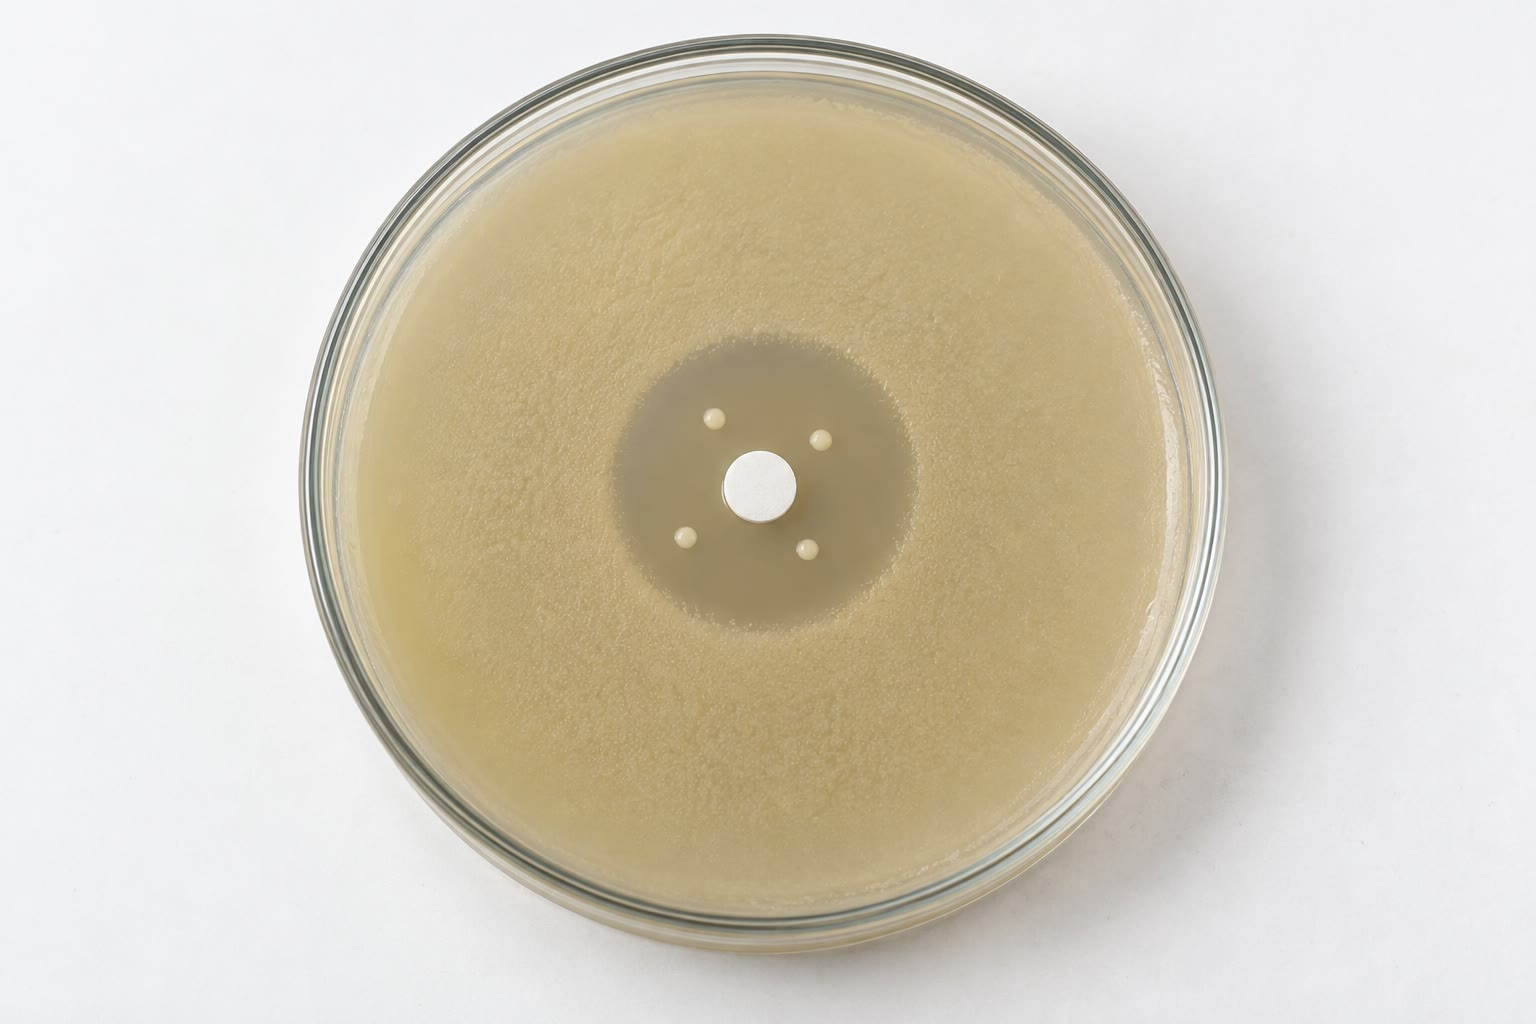
\includegraphics[width=0.5\linewidth]{images/book4/ai/b4-03-luria-plate.jpg}

{\small जीवाणुओं की चटाई पर एक प्रतिजैविक चक्रिका: स्वच्छ क्षेत्र वह है
जहाँ चक्रिका से विसरित होती औषधि ने संवेदी कोशिकाएँ मार डालीं, और उसके
भीतर के निवह उन प्रतिरोधी उत्परिवर्तियों से उगे जो चक्रिका रखे जाने से
पहले ही मौजूद थे।}
\end{omfigure}

\begin{proposition}[मरम्मत और उसकी सीमाएँ]\label{prop:b2:genome-diversification:repair}
\index{DNA मरम्मत}
कोशिका अधिकांश क्षति को \omterm{def:b2:genome-diversification:mutation}{उत्परिवर्तन} बनने से पहले ही सुधार देती है।
\emph{बेमेल-मरम्मत} नए बने रज्जु से ग़लत क्षारक हटा देती है।
\emph{क्षारक-उच्छेदन मरम्मत} एक ही क्षतिग्रस्त क्षारक (कोई यूरेसिल, कोई
ऑक्सीकृत ग्वानीन) काटकर निकालती है और रिक्ति भर देती है; इसीलिए DNA में
यूरेसिल के बजाय थाइमीन है: DNA में कोई यूरेसिल केवल विऐमीनित साइटोसीन ही
हो सकता है, और वह पराया पहचान लिया जाता है। \emph{न्यूक्लियोटाइड-उच्छेदन
मरम्मत} किसी भारी-भरकम क्षति के, जैसे थाइमीन द्विलक के, चारों ओर से एक
दर्जन क्षारक का टुकड़ा हटा देती है; जिन लोगों में यह नहीं है
(ज़ेरोडर्मा पिग्मेंटोसम) उन्हें साधारण धूप से ही त्वचा-कैंसर हो जाते
हैं। \emph{पुनर्संयोजी मरम्मत} टूटे गुणसूत्र को उसकी सहोदरी प्रति से
फिर गढ़ देती है। जो मरम्मत से बच जाए, या जिसकी मरम्मत ग़लत हो जाए, वही
\omterm{def:b2:genome-diversification:mutation}{उत्परिवर्तन} है --- और जिस कोशिका ने कोई मरम्मत तंत्र खो दिया हो (कोई
\emph{उत्परिवर्तक}) वह सौ गुना तेज़ उत्परिवर्तित होती है, जो दबाव में
अल्पकालिक लाभ और दीर्घकालिक बोझ है। मरम्मत की क्रियाविधियों पर वर्ष 3 के
खंड में विस्तार से विचार है।
\end{proposition}

\section{जो जीन चलते हैं}

\begin{definition}[स्थानांतरणीय तत्व]\label{def:b2:genome-diversification:transposon}
\index{ट्रांसपोसॉन}\index{रेट्रोट्रांसपोसॉन}
\emph{स्थानांतरणीय तत्व} DNA का ऐसा खंड है जो जीनोम में किसी नई स्थिति
पर जा सकता है। \emph{DNA ट्रांसपोसॉन} कोई \emph{ट्रांसपोसेज़} कूटबद्ध
करते हैं जो उस तत्व को काटकर निकालता है और कहीं और चिपका देता है (या
वहाँ उसकी प्रति बना देता है); जीवाणुओं के अंतर्वेशन अनुक्रम सबसे सरल
हैं (दो प्रतिलोमित पुनरावृत्तियों के बीच एक ट्रांसपोसेज़ जीन), और
संयुक्त ट्रांसपोसॉन उनमें से दो के बीच अतिरिक्त जीन --- प्रायः
प्रतिजैविक प्रतिरोध --- ढोते हैं। \emph{रेट्रोट्रांसपोसॉन} किसी RNA
मध्यवर्ती के रास्ते नक़ल-और-चिपकाओ ढंग से चलते हैं, और वह RNA किसी
प्रतिलोम ट्रांसक्रिप्टेज़ से फिर DNA में उतारी जाती है; वे अपना पुराना
स्थल कभी नहीं छोड़ते और इसलिए जमा होते जाते हैं। किसी जीन में उतरा तत्व
उसे बिगाड़ देता है; किसी के पास उतरे तो उसकी अभिव्यक्ति बदल सकता है; और
एक ही गुणसूत्र में दो प्रतियाँ \omterm{prop:b2:genome-diversification:duplication}{असमान जीन-विनिमय} के लिए स्थल दे देती हैं।
ट्रांसपोसॉन और उनके अवशेष मानव जीनोम का आधा और मक्का के जीनोम का अस्सी
प्रतिशत बनाते हैं; अधिकांश अब निश्चल हैं।
\end{definition}
\begin{proof}[प्रमाण-सामग्री]
मक्लिंटॉक ने (1940--1950 के दशकों में) मक्का के उन दानों का अध्ययन किया
जिनका बैंगनी रंजक कुछ कोशिकाओं में खो जाता था और दूसरी में लौट आता था,
जिससे दाने चितकबरे हो जाते थे। उन्होंने प्रजनन और गुणसूत्र-प्रेक्षण से
दिखाया कि यह अस्थिरता ऐसे तत्व (\emph{डिसोसिएशन}) से होती थी जो जहाँ
बैठता वहीं गुणसूत्र तोड़ देता और किसी दूसरे तत्व (\emph{ऐक्टिवेटर}) के
नियंत्रण में स्थानों के बीच घूमता; और यह कि तत्व जीन में बैठे तो जीन चुप
हो जाता और उसके निकलते ही फिर चालू हो जाता। उन्होंने निष्कर्ष निकाला कि
जीन अपनी स्थिति बदल सकते हैं; यह विचार बीस वर्ष बाद ही स्वीकारा गया, जब
जीवाणुओं के अंतर्वेशन अनुक्रम मिले, और उन्हें 1983 में नोबेल पुरस्कार
दिला गया।
\end{proof}

\begin{omfigure}
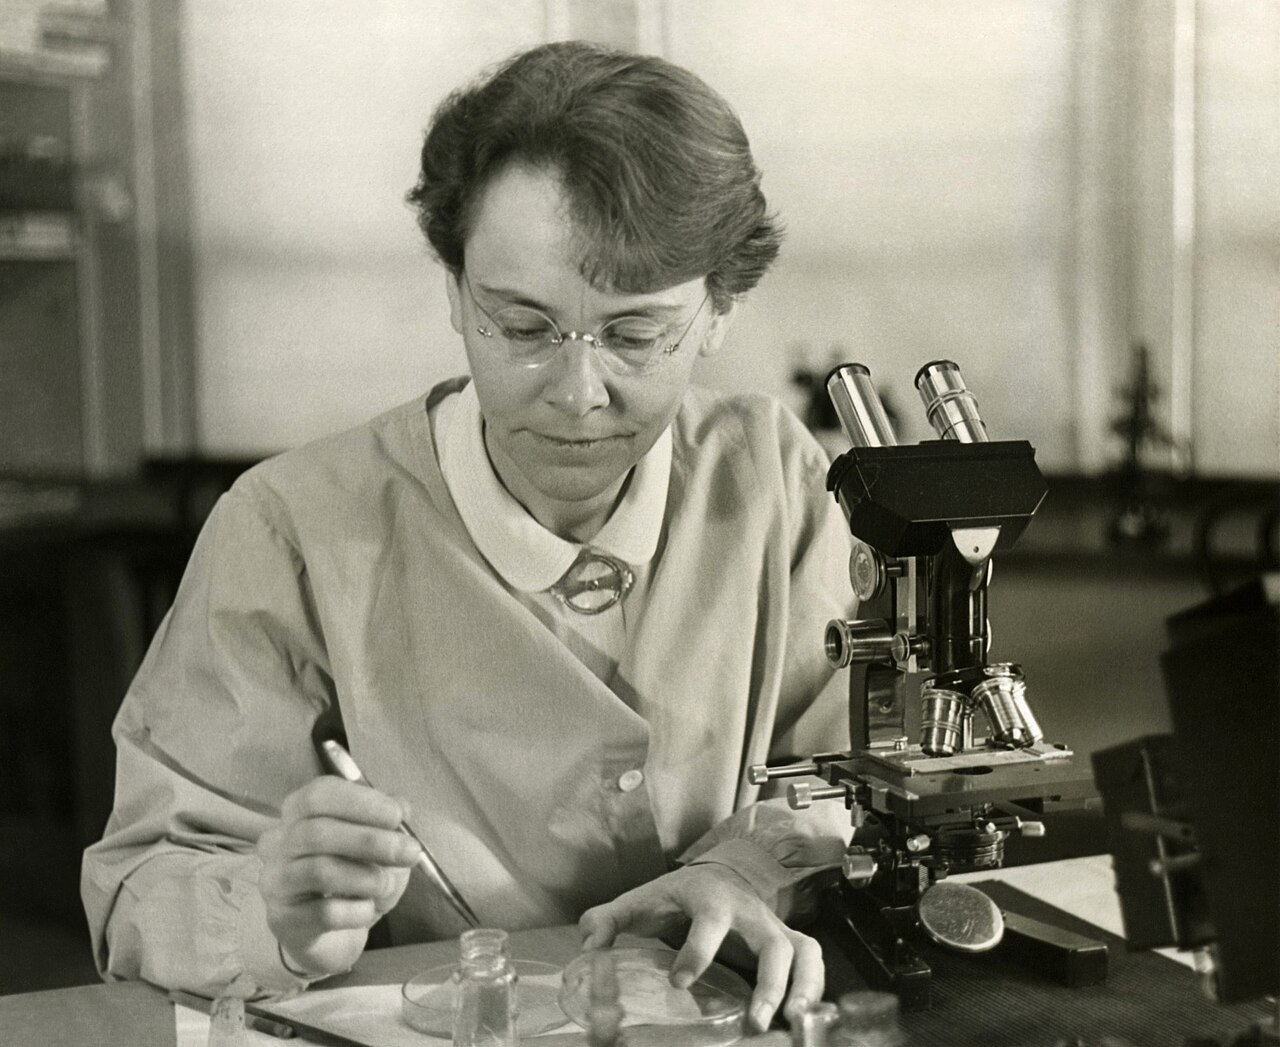
\includegraphics[width=0.4\linewidth]{images/book4/mcclintock.jpg}\hspace{0.04\linewidth}
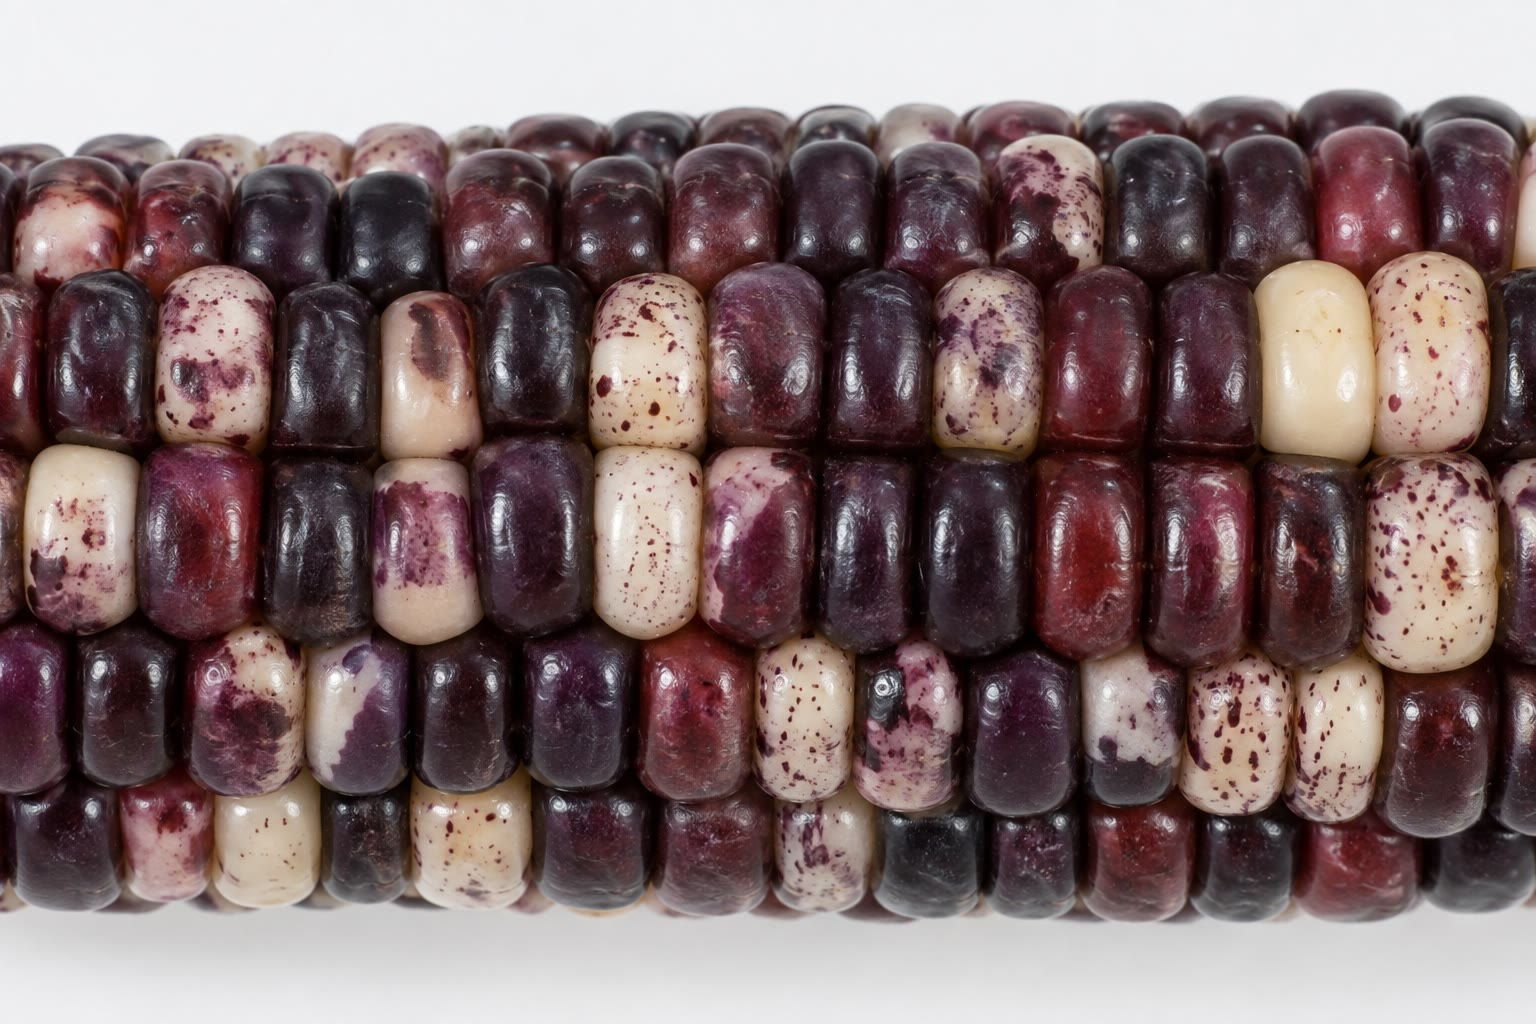
\includegraphics[width=0.5\linewidth]{images/book4/ai/b4-03-maize-kernels.jpg}

{\small बारबरा मक्लिंटॉक, और वे दाने जो उन्हें स्थानांतरणीय तत्वों
तक ले गए: कोई अंतर्वेशित तत्व बैंगनी रंजक का जीन बंद कर देता है और, तत्व
के कूदकर निकल जाने पर, कोशिका-दर-कोशिका उसे फिर चालू कर देता है, और यों
चित्तियाँ तथा खंड छूट जाते हैं।}
\end{omfigure}

\begin{omfigure}
\begin{tikzpicture}[every node/.style={font=\scriptsize}]
  % cut and paste
  \begin{scope}
    \draw[very thick, gray] (0,1.2) -- (4.5,1.2);
    \fill[omThm!70] (0.8,1.05) rectangle (1.8,1.35); \node[white, font=\tiny] at (1.3,1.2) {Tn};
    \draw[very thick, gray] (0,0) -- (4.5,0);
    \fill[omThm!70] (2.8,-0.15) rectangle (3.8,0.15); \node[white, font=\tiny] at (3.3,0) {Tn};
    \draw[->, thick, omThm] (1.3,1.0) .. controls (1.3,0.5) and (3.3,0.7) .. (3.3,0.2);
    \draw[dashed, gray] (0.8,1.2) -- (1.8,1.2);
    \node[align=center] at (2.25,-0.6) {काटो और चिपकाओ (DNA ट्रांसपोसॉन):\\तत्व अपना पुराना स्थल छोड़ देता है};
  \end{scope}
  % copy and paste
  \begin{scope}[xshift=7.5cm]
    \draw[very thick, gray] (0,1.2) -- (4.5,1.2);
    \fill[omProp!80] (0.8,1.05) rectangle (1.8,1.35); \node[white, font=\tiny] at (1.3,1.2) {RT};
    \draw[very thick, gray] (0,0) -- (4.5,0);
    \fill[omProp!80] (2.8,-0.15) rectangle (3.8,0.15); \node[white, font=\tiny] at (3.3,0) {RT};
    \draw[->, thick, omProp] (1.3,1.0) .. controls (1.3,0.5) and (3.3,0.7) .. (3.3,0.2);
    \node[omProp, anchor=west, align=left] at (3.6,0.75) {RNA प्रति,\\प्रतिलोम अनुलेखित};
    \node[align=center] at (2.25,-0.6) {नक़ल करो और चिपकाओ (रेट्रोट्रांसपोसॉन):\\पुरानी प्रति बनी रहती है, संख्या बढ़ती है};
  \end{scope}
\end{tikzpicture}

{\small चलने के दो ढंग। कोई DNA \omterm{def:b2:genome-diversification:transposon}{ट्रांसपोसॉन} काटकर निकाला और
फिर अंतर्वेशित किया जाता है; कोई \omterm{def:b2:genome-diversification:transposon}{रेट्रोट्रांसपोसॉन} अनुलेखित होता है, फिर
DNA में उतारा जाता है और कहीं और अंतर्वेशित किया जाता है, ताकि उसकी
प्रतियाँ जमा होती जाएँ।}
\end{omfigure}

\begin{definition}[क्षैतिज जीन हस्तांतरण]\label{def:b2:genome-diversification:hgt}
\index{क्षैतिज जीन हस्तांतरण}\index{रूपांतरण}\index{संयुग्मन!जीवाणुओं में}\index{पारक्रमण}
\omterm{def:b2:unicellular-diversity:prokaryote}{प्राक्केंद्रकी} अपने माता-पिता से भिन्न कोशिकाओं से तीन रास्तों से जीन
प्राप्त करते हैं। \emph{रूपांतरण}: कोई कोशिका अपने परिवेश से नंगा DNA
ग्रहण कर लेती है (जो मरी हुई कोशिकाओं ने छोड़ा है) और उसे अपने गुणसूत्र
में पुनर्संयोजित कर लेती है; कुछ जातियाँ स्वभाव से ही सक्षम होती हैं,
और न्यूमोकॉकस इसी रास्ते से संपुट के जीन बदलते हैं। \emph{संयुग्मन}:
कोई दाता, जो कोई संयुग्मी \omterm{def:b2:unicellular-diversity:prokaryote}{प्लास्मिड} (\emph{E.~coli} का F कारक) ढोता है,
एक पिलस बनाता है, किसी ग्राही को पास खींचता है, और \omterm{def:b2:unicellular-diversity:prokaryote}{प्लास्मिड} को लोटता
वृत्त ढंग से प्रतिकृत करते हुए उसका एक रज्जु किसी छिद्र से पार भेज देता
है; यदि वह \omterm{def:b2:unicellular-diversity:prokaryote}{प्लास्मिड} गुणसूत्र में समाकलित हो चुका हो (कोई Hfr विभेद), तो
गुणसूत्रीय जीन उसके पीछे क्रम से हस्तांतरित होते हैं, और हर एक के प्रवेश
का समय गुणसूत्र का मानचित्र बना देता है। \emph{पारक्रमण}: कोई
जीवाणुभोजी भूल से पोषी DNA का एक टुकड़ा संवेष्टित कर लेता है और अगली
कोशिका को संक्रमित करते समय उसमें उड़ेल देता है। मिलकर ये रास्ते
अस्पतालों के भीतर कुछ ही वर्षों में प्रतिरोध के जीन जातियों के बीच हिला
देते हैं, और भूवैज्ञानिक काल में उपापचयी जीनों को पूरे जीवाणु-वृक्ष के
आरपार ले जा चुके हैं, इसलिए किसी \omterm{def:b2:unicellular-diversity:prokaryote}{प्राक्केंद्रकी} की वंशावली उतनी ही एक
जाल है जितनी एक वृक्ष
(\cref{ch:b2:phylogenetic-trees})।
\end{definition}
\begin{proof}[प्रमाण-सामग्री]
लेडरबर्ग और टेटम (1946) ने \emph{E.~coli} के दो विभेद मिलाए, जिनमें से
हर एक दो अलग-अलग पोषक नहीं बना सकता था, और मिश्रण को ऐसे न्यूनतम माध्यम
पर बोया जिस पर कोई भी अकेला नहीं उग सकता था: कोई एक करोड़ कोशिकाओं में
एक की दर से ऐसे निवह उग आए जो चारों बना सकते थे --- यानी पुनर्संयोजी।
डेविस (1950) ने वही प्रयोग विभेदों को ऐसे निस्यंदक से अलग रखकर दोहराया
जो अणु तो जाने देता था पर कोशिकाएँ नहीं: कोई पुनर्संयोजी नहीं मिला,
इसलिए संपर्क आवश्यक था। फिर हेस ने दिखाया कि हस्तांतरण एकतरफ़ा है, दाता
से ग्राही की ओर, और वोलमैन तथा जैकब (1956) ने अंतराल पर किसी मिश्रक में
संगम तोड़कर पाया कि दाता के जीन ग्राही में एक निश्चित क्रम में, एक के
बाद एक, कोई सौ मिनट में प्रवेश करते हैं।
\end{proof}

\begin{omfigure}
\begin{minipage}[b]{0.56\linewidth}\centering
\begin{tikzpicture}[every node/.style={font=\scriptsize}]
  % donor
  \draw[thick, fill=omDef!8] (0,0) ellipse (1.5 and 0.75);
  \draw[thick, omDef] (0.2,0) circle (0.45);
  \draw[thick, omThm] (-0.9,0.1) circle (0.22);
  \node[anchor=south] at (0,1.25) {दाता $F^+$};
  \draw[omThm] (-0.9,-0.12) -- (-1.1,-1.0) node[below] {F प्लास्मिड};
  \draw[omDef] (0.4,-0.4) -- (0.6,-1.0) node[below] {गुणसूत्र};
  % recipient
  \draw[thick, fill=omDef!8] (5,0) ellipse (1.5 and 0.75);
  \draw[thick, omDef] (5.2,0) circle (0.45);
  \node[anchor=south] at (5,1.25) {ग्राही $F^-$};
  % pilus
  \draw[very thick, omThm] (1.5,0) -- (3.5,0);
  \node[omThm, below] at (2.5,-0.05) {पिलस};
  % single strand transferred
  \draw[->, thick, omThm, dashed] (-0.7,0.15) .. controls (1.0,0.7) and (3.0,0.7) .. (4.1,0.4);
  \node[omThm, anchor=south] at (2.5,0.7) {लोटते वृत्त से एक रज्जु की नक़ल};
  \draw[thick, omThm, dashed] (4.1,0.2) circle (0.2);
\end{tikzpicture}
\end{minipage}\hfill
\begin{minipage}[b]{0.42\linewidth}\centering
\begin{tikzpicture}
\begin{axis}[
  width=\linewidth, height=4.6cm,
  axis x line=bottom, axis y line=left,
  xmin=0, xmax=40, ymin=0, ymax=1.1,
  xlabel={मिश्रण से पहले के मिनट}, ylabel={पुनर्संयोजी (सापेक्ष)},
  xlabel style={font=\scriptsize, at={(axis description cs:0.5,-0.18)}, anchor=north},
  ylabel style={font=\scriptsize},
  tick label style={font=\scriptsize}, xtick={0,10,20,30,40}, ytick={0,0.5,1},
  legend style={font=\scriptsize, at={(0.97,0.08)}, anchor=south east, draw=none},
  clip=false,
]
\addplot[very thick, omDef, domain=8:40, samples=40] {1-exp(-(x-8)/5)};
\addlegendentry{\emph{thr}, \qty{8}{min} पर प्रवेश}
\addplot[very thick, omProp, domain=17:40, samples=40] {1-exp(-(x-17)/5)};
\addlegendentry{\emph{lac}, \qty{17}{min}}
\addplot[very thick, omThm, domain=25:40, samples=40] {1-exp(-(x-25)/5)};
\addlegendentry{\emph{gal}, \qty{25}{min}}
\end{axis}
\end{tikzpicture}
\end{minipage}

{\small बाएँ: संयुग्मन --- दाता अपने F \omterm{def:b2:unicellular-diversity:prokaryote}{प्लास्मिड}
के एक रज्जु की नक़ल करते हुए उसे पिलस संधि से पार भेजता है। दाएँ: किसी
Hfr दाता के साथ संगम-भंग प्रयोग: हर गुणसूत्रीय जीन पुनर्संयोजियों में
किसी अभिलाक्षणिक समय पर दिखने लगता है, और यही गुणसूत्र का मानचित्र मिनटों
में बना देता है।}
\end{omfigure}

\begin{omfigure}
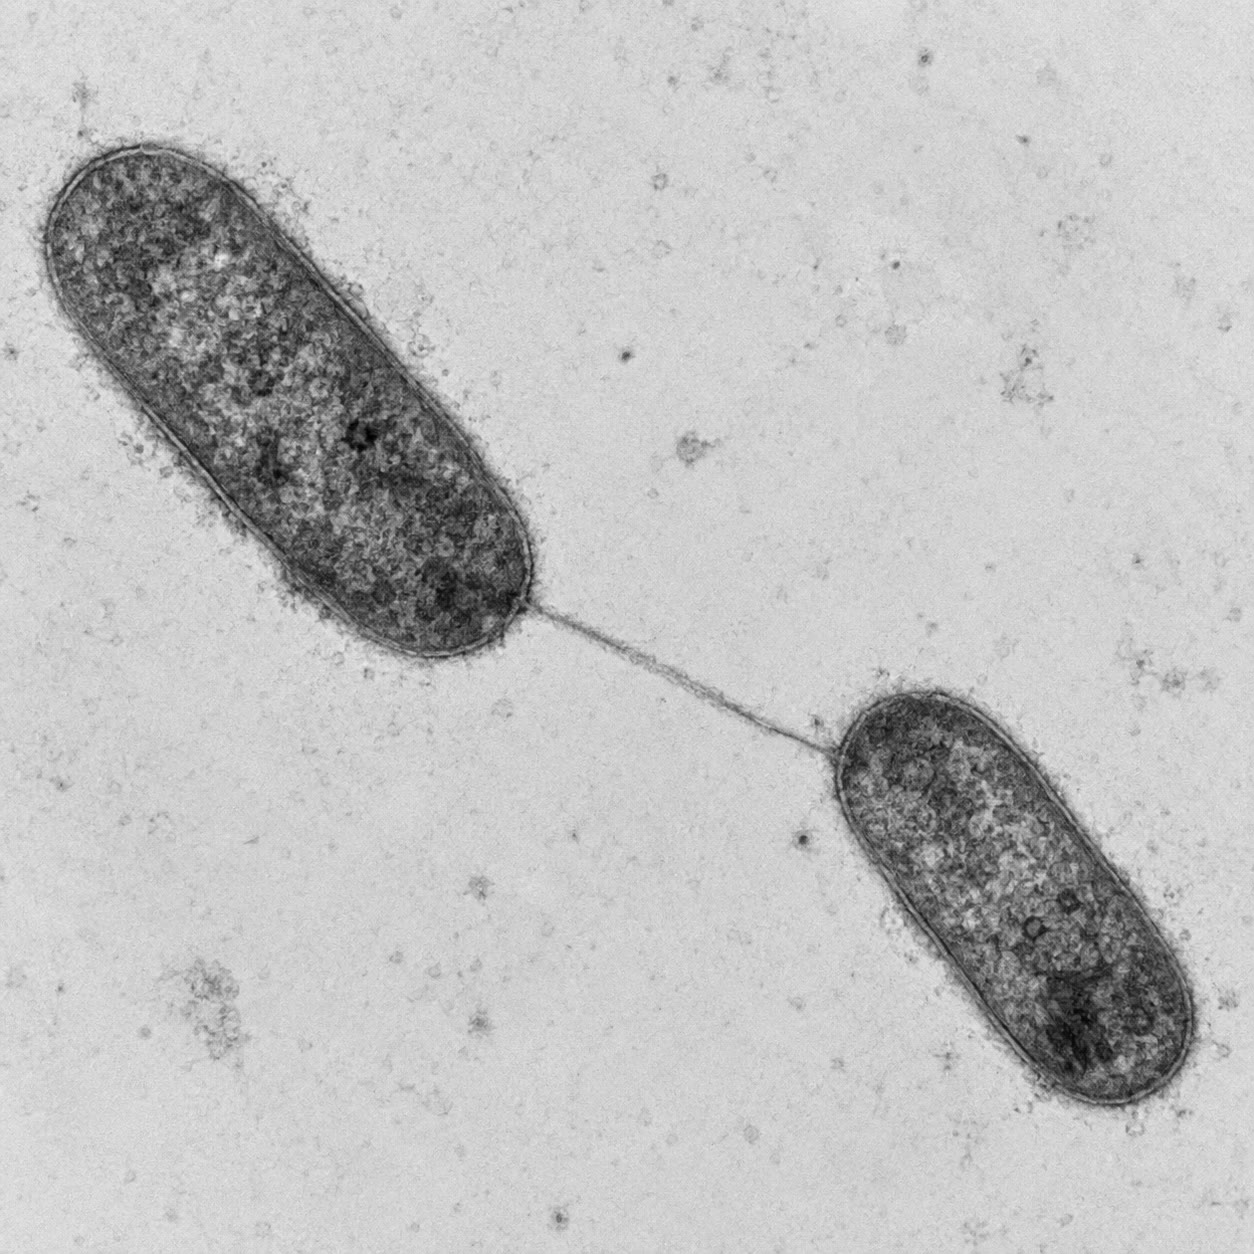
\includegraphics[width=0.42\linewidth]{images/book4/ai/b4-03-conjugation-tem.jpg}

{\small संयुग्मी पिलस से जुड़े दो जीवाणु, पारेषण इलेक्ट्रॉन
सूक्ष्मदर्शन में: वही पुल जिससे \omterm{def:b2:unicellular-diversity:prokaryote}{प्लास्मिड}
पार जाता है।}
\end{omfigure}

\begin{example}[चलता-फिरता प्रतिरोध]\label{ex:b2:genome-diversification:resistance}
प्रतिरोध का कोई जीन प्रायः एक ही बार उठता है, किसी \omterm{def:b2:genome-diversification:mutation}{उत्परिवर्तन} से या उस
मृदा-जीवाणु से जो वह प्रतिजैविक बनाता है, और फिर यात्रा करता है: किसी
गुणसूत्र से किसी \omterm{def:b2:genome-diversification:transposon}{ट्रांसपोसॉन} पर, उस \omterm{def:b2:genome-diversification:transposon}{ट्रांसपोसॉन} से किसी
संयुग्मी \omterm{def:b2:unicellular-diversity:prokaryote}{प्लास्मिड} पर, उस \omterm{def:b2:unicellular-diversity:prokaryote}{प्लास्मिड} से संयुग्मन द्वारा जातियों के आरपार
और \omterm{def:b2:genome-diversification:hgt}{पारक्रमण} द्वारा विभेदों के आरपार, और \omterm{def:b2:genome-diversification:hgt}{रूपांतरण}
द्वारा फिर किसी गुणसूत्र में। एक साथ पाँच-छह प्रतिरोध ढोते \omterm{def:b2:unicellular-diversity:prokaryote}{प्लास्मिड}
(जो \emph{इंटीग्रॉनों} में जुड़ते हैं, और वे जीन-कैसेट पकड़ते हैं) जापान
में 1950 के दशक में मिले, यानी औषधियों के प्रचलन में आने के कुछ ही वर्ष
बाद; कार्बापेनेमेज़ NDM-1 का जीन, जो पहली बार 2008 में दिखा, तीन वर्षों
के भीतर किसी \omterm{def:b2:unicellular-diversity:prokaryote}{प्लास्मिड} पर हर महाद्वीप तक पहुँच गया। प्रतिरोध का
विकास अधिकतर नए जीनों का विकास नहीं, बल्कि पुराने जीनों का चलना है।
\end{example}

\section{द्विगुणन: जीन और जीनोम}

\begin{proposition}[जीन द्विगुणन और जीन कुल]\label{prop:b2:genome-diversification:duplication}
\index{जीन द्विगुणन}\index{जीन कुल}\index{असमान जीन-विनिमय}
जब दो मिलते-जुलते अनुक्रम किसी गुणसूत्र पर अनुक्रमशः बैठे हों, तो
अर्धसूत्री विभाजन में समजात बेतरतीब युग्मित हो सकते हैं और असमान रूप से
जीन-विनिमय कर सकते हैं, जिससे एक उत्पाद तीन प्रतियाँ ढोता है और दूसरा
एक। द्विगुणित जीन अनावश्यक होता है: एक प्रति पुराना काम सँभाले रख सकती
है जबकि दूसरी स्वतंत्र रूप से \omterm{def:b2:genome-diversification:mutation}{उत्परिवर्तन} जमा करती जाए --- और वह
प्रायः किसी \emph{आभासी जीन} में क्षीण हो जाती है, कभी-कभार कोई नया
कार्य पा लेती है (\emph{नवकार्यन}) या पुराने कार्य का एक हिस्सा
(\emph{उपकार्यन})। करोड़ों वर्षों तक दोहराए जाने पर यही
\emph{\omterm{prop:b2:genome-diversification:duplication}{जीन कुल}} गढ़ता है: ग्लोबिन (एक ही पूर्वज जीन से मायोग्लोबिन,
$\alpha$ गुच्छ और $\beta$ गुच्छ बने, जिनके भ्रूणीय, गर्भस्थ और वयस्क
सदस्य बारी-बारी अभिव्यक्त होते हैं), गंध-ग्राही (चूहे में एक हज़ार
जीन), होमियोबॉक्स जीन, लेंस के क्रिस्टलिन। किसी जीनोम के अधिकांश जीन
किसी न किसी कुल के हैं, और द्विगुणन नए जीनों का मुख्य स्रोत है।
\end{proposition}
\begin{proof}[प्रमाण-सामग्री]
गुणसूत्र 11 पर मानव $\beta$-ग्लोबिन गुच्छ में पाँच
क्रियाशील जीन ($\varepsilon$, $^{G}\gamma$, $^{A}\gamma$,
$\delta$, $\beta$) और एक आभासी जीन हैं, उसी क्रम में जिसमें वे विकास के
दौरान चालू होते हैं, सबकी वही एक्सॉन--इंट्रॉन संरचना है, और उनके अनुक्रम
जितने हाल में अलग हुए उतने ही अधिक मिलते-जुलते हैं; गुणसूत्र 16 पर
$\alpha$ गुच्छ की भी वही स्थापत्य-रचना है। लगभग एक जैसी प्रतियों के बीच
\omterm{prop:b2:genome-diversification:duplication}{असमान जीन-विनिमय} से बने एक या अधिक $\alpha$ जीनों के विलोपन आम हैं
और $\alpha$-थैलेसीमिया कराते हैं; और उसका प्रतिलोम उत्पाद, यानी तीन
$\alpha$ जीन वाला गुणसूत्र, उन्हीं आबादियों में मिलता है।
\end{proof}

\begin{omfigure}
\begin{tikzpicture}[every node/.style={font=\scriptsize}]
  % unequal crossing over
  \begin{scope}
    \draw[very thick, gray] (0,1.2) -- (5,1.2);
    \fill[omDef!70] (1.0,1.05) rectangle (2.0,1.35); \fill[omDef!70] (2.4,1.05) rectangle (3.4,1.35);
    \draw[very thick, gray] (0,0) -- (5,0);
    \fill[omDef!70] (1.0,-0.15) rectangle (2.0,0.15); \fill[omDef!70] (2.4,-0.15) rectangle (3.4,0.15);
    \node[above] at (1.5,1.35) {A}; \node[above] at (2.9,1.35) {A$'$};
    \draw[very thick, omThm] (2.9,1.05) -- (1.5,0.15);
    \node[align=center] at (2.5,-0.6) {बेमेल युग्मित समजात\\असमान जीन-विनिमय करते हैं};
    \draw[->, thick, gray] (5.3,0.6) -- (6.1,0.6);
    % products
    \draw[very thick, gray] (6.5,1.2) -- (11.5,1.2);
    \fill[omDef!70] (7.5,1.05) rectangle (8.5,1.35); \fill[omDef!70] (8.9,1.05) rectangle (9.9,1.35); \fill[omDef!70] (10.3,1.05) rectangle (11.3,1.35);
    \node[above] at (9.4,1.35) {तीन प्रतियाँ};
    \draw[very thick, gray] (6.5,0) -- (11.5,0);
    \fill[omDef!70] (7.5,-0.15) rectangle (8.5,0.15);
    \node[above] at (8.0,0.15) {एक प्रति};
  \end{scope}
  % globin family tree
  \begin{scope}[yshift=-3.6cm]
    \draw[thick] (2,2.2) -- (2,1.7);
    \draw[thick] (0.5,1.7) -- (3.5,1.7);
    \draw[thick] (0.5,1.7) -- (0.5,0.4); \node[below] at (0.5,0.4) {मायोग्लोबिन};
    \draw[thick] (3.5,1.7) -- (3.5,1.2);
    \draw[thick] (2.3,1.2) -- (4.7,1.2);
    \draw[thick] (2.3,1.2) -- (2.3,0.4); \node[below] at (2.3,0.4) {$\alpha$ कुल};
    \draw[thick] (4.7,1.2) -- (4.7,0.9);
    \draw[thick] (3.6,0.9) -- (5.8,0.9);
    \draw[thick] (3.6,0.9) -- (3.6,0.4); \node[below] at (3.6,0.4) {$\varepsilon,\gamma$};
    \draw[thick] (5.8,0.9) -- (5.8,0.7);
    \draw[thick] (5.2,0.7) -- (6.4,0.7);
    \draw[thick] (5.2,0.7) -- (5.2,0.4); \node[below] at (5.2,0.4) {$\delta$};
    \draw[thick] (6.4,0.7) -- (6.4,0.4); \node[below] at (6.4,0.4) {$\beta$};
    \node[anchor=west, align=left] at (7.2,1.7) {एक पूर्वज ग्लोबिन जीन के द्विगुणन:\\कशेरुकियों से पहले (मायोग्लोबिन/हीमोग्लोबिन),\\$\sim$45 करोड़ वर्ष पहले ($\alpha$/$\beta$),\\फिर $\beta$ गुच्छ के भीतर (भ्रूणीय, गर्भस्थ, वयस्क)};
    \node[anchor=east, gray] at (1.9,2.1) {पूर्वज ग्लोबिन};
  \end{scope}
\end{tikzpicture}

{\small ऊपर: बेमेल युग्मित अनुक्रमिक प्रतियों के बीच \omterm{prop:b2:genome-diversification:duplication}{असमान जीन-विनिमय}
एक ऐसा गुणसूत्र बनाता है जिसमें तीन प्रतियाँ हैं और एक ऐसा जिसमें एक।
नीचे: ग्लोबिन कुल, जो क्रमिक द्विगुणनों और अपसरण से गढ़ा गया।}
\end{omfigure}

\begin{definition}[बहुगुणिता]\label{def:b2:genome-diversification:polyploidy}
\index{बहुगुणिता}\index{विषमबहुगुणित}\index{समबहुगुणित}
कोई \emph{बहुगुणित} दो से अधिक पूरे गुणसूत्र-समुच्चय ढोता है।
कोई \emph{समबहुगुणित} एक ही जाति से कई समुच्चय रखता है (कोई विफल
अर्धसूत्री विभाजन द्विगुणित युग्मक देता है; ऐसे दो युग्मक कोई
चतुर्गुणित देते हैं); कोई \emph{विषमबहुगुणित} किसी संकरण के बाद दो
जातियों के समुच्चय जोड़ लेता है। द्विगुणित संकर AB, जिसके किसी भी
गुणसूत्र का कोई समजात नहीं है, अर्धसूत्री विभाजन में उन्हें युग्मित नहीं
कर सकता और बंध्य है; यदि उसका जीनोम दुगुना होकर AABB हो जाए, तो हर
गुणसूत्र को फिर एक साथी मिल जाता है, अर्धसूत्री विभाजन चल पड़ता है, और
वह नया पौधा उर्वर है --- पर किसी भी जनक से फिर संकरण नहीं कर सकता (कोई
AAB संतान बंध्य होती है)। इस तरह बहुगुणिता एक ही पग में नई जाति बना देती
है, और सपुष्पक जातियों में से लगभग एक तिहाई इसी तरह उठी हैं: रोटी का गेहूँ
तीन घासों का षड्गुणित AABBDD है, बाग़ की स्ट्रॉबेरी अष्टगुणित, कपास और
तंबाकू विषमचतुर्गुणित, और कशेरुकी वंशक्रम ने भी अपने उद्गम के पास अपना
जीनोम दो बार दुगुना किया। बहुगुणित प्रायः अपने द्विगुणित पूर्वजों से बड़े
होते हैं (अधिक DNA, बड़ी कोशिकाएँ) और प्रजनकों को बहुत प्रिय हैं।
\end{definition}

\begin{omfigure}
\begin{tikzpicture}[every node/.style={font=\scriptsize}]
  \node[draw, rounded corners, fill=omDef!10, align=center] (a) at (0,0) {\emph{T.~urartu}\\AA, $2n = 14$};
  \node[draw, rounded corners, fill=omDef!10, align=center] (b) at (3.4,0) {\emph{Aegilops}\\BB, $2n = 14$};
  \node[draw, rounded corners, fill=omProp!15, align=center] (ab) at (1.7,-1.5) {संकर AB\\$n = 14$, बंध्य};
  \node[draw, rounded corners, fill=omExo!25, align=center] (aabb) at (1.7,-3.1) {एमर गेहूँ AABB\\$2n = 28$, उर्वर};
  \node[draw, rounded corners, fill=omDef!10, align=center] (d) at (6.4,-3.1) {\emph{Ae.~tauschii}\\DD, $2n = 14$};
  \node[draw, rounded corners, fill=omProp!15, align=center] (abd) at (4.0,-4.6) {संकर ABD\\$3n = 21$, बंध्य};
  \node[draw, rounded corners, fill=omExo!25, align=center] (abd2) at (4.0,-6.1) {रोटी का गेहूँ AABBDD\\$2n = 42$, उर्वर};
  \draw[->, thick] (a) -- (ab); \draw[->, thick] (b) -- (ab);
  \draw[->, thick] (ab) -- (aabb) node[midway, right] {जीनोम का दुगुना होना};
  \draw[->, thick] (aabb) -- (abd); \draw[->, thick] (d) -- (abd);
  \draw[->, thick] (abd) -- (abd2) node[midway, right] {जीनोम का दुगुना होना};
  \node[anchor=west, align=left, gray] at (7.8,-1.5) {हर संकरण अयुग्मित गुणसूत्रों वाला\\एक बंध्य पौधा देता है;\\हर दुगुनापन युग्मन और उर्वरता\\लौटा देता है --- और ऐसी जाति\\बना देता है जो पीछे संकरण नहीं कर सकती};
\end{tikzpicture}

{\small रोटी के गेहूँ का उद्गम: दो संकरण, और हर एक के बाद जीनोम का
दुगुना होना, जिन्होंने लगभग दस हज़ार वर्षों में तीन द्विगुणित घासों से
एक षड्गुणित गढ़ दिया।}
\end{omfigure}

\begin{omfigure}
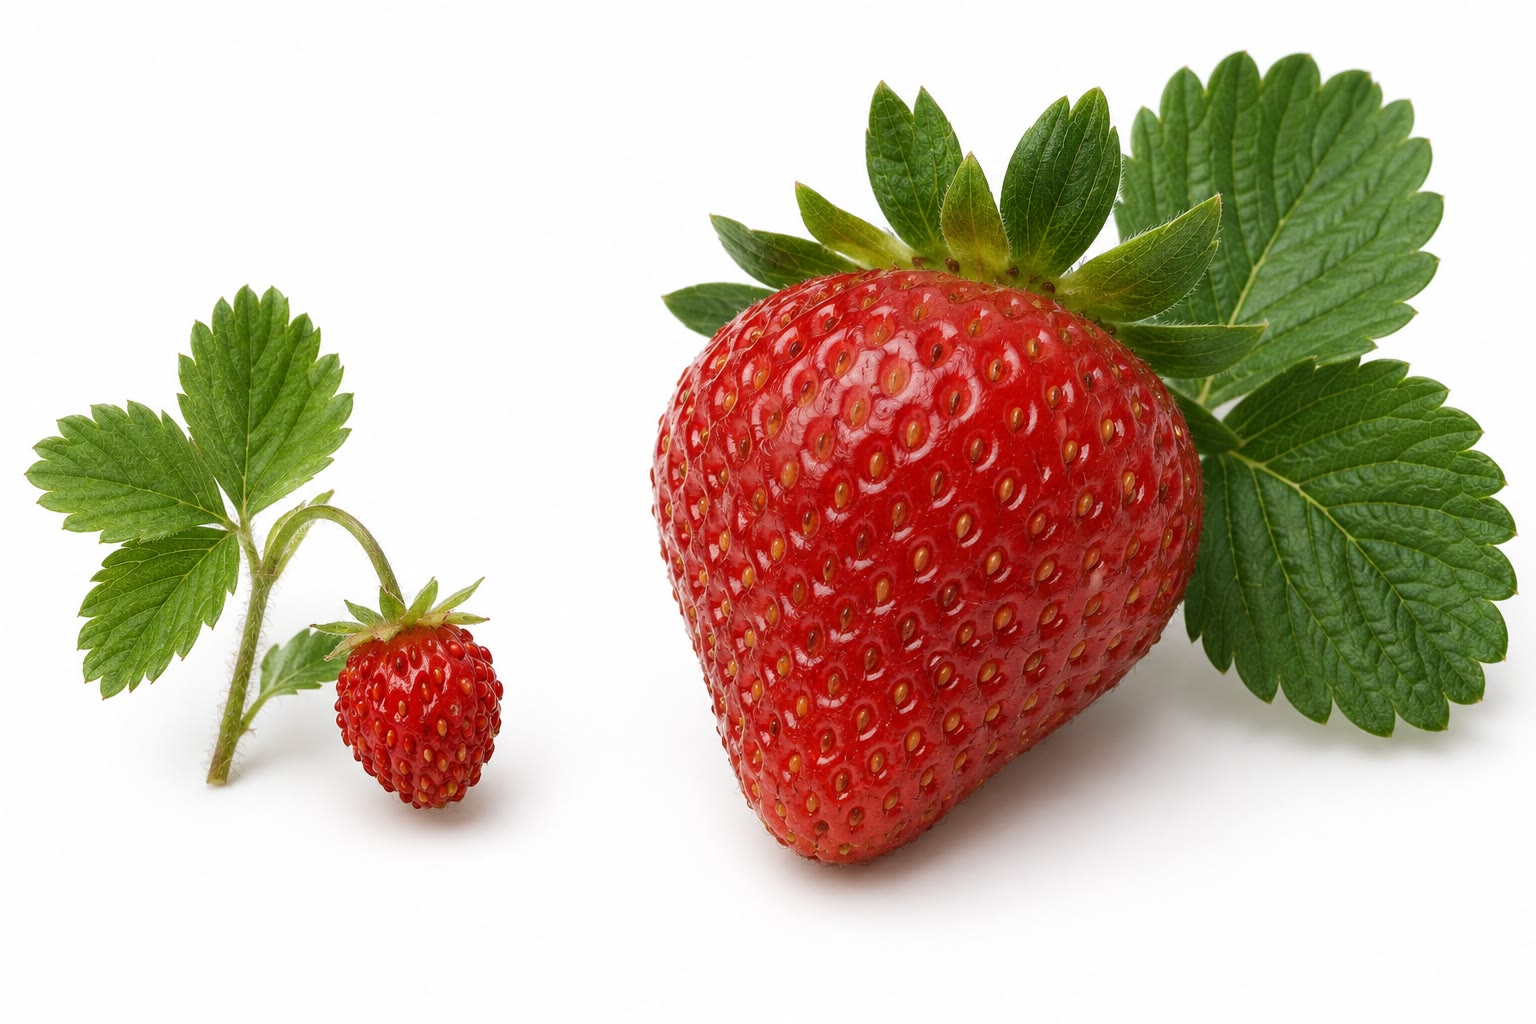
\includegraphics[width=0.55\linewidth]{images/book4/ai/b4-03-polyploid-strawberries.jpg}

{\small एक जंगली द्विगुणित स्ट्रॉबेरी और खेती वाली अष्टगुणित: वह
\omterm{def:b2:genome-diversification:polyploidy}{बहुगुणित}, जिसकी हर कोशिका में चार गुना DNA है, बड़े फल वाला बड़ा
पौधा है।}
\end{omfigure}

\section{यादृच्छिकता और दर}

\begin{proposition}[उत्परिवर्तन आवश्यकता के प्रति यादृच्छिक है]\label{prop:b2:genome-diversification:random}
\index{उत्परिवर्तन!की यादृच्छिकता}
\omterm{thm:b2:genome-diversification:luria}{उच्चावचन परीक्षण} और प्रतिलिपि-बुवाई दिखाते हैं कि किसी नए पर्यावरण में
उपयोगी कोई \omterm{def:b2:genome-diversification:mutation}{उत्परिवर्तन} उसी दर से उठता है, चाहे वह पर्यावरण उपस्थित हो या
न हो: पर्यावरण \omterm{def:b2:genome-diversification:mutation}{उत्परिवर्तनों} में से चुनता है, उन्हें बुलाता नहीं।
\omterm{def:b2:genome-diversification:mutation}{उत्परिवर्तन} हर अर्थ में यादृच्छिक नहीं है --- संक्रमण पर्यावर्तनों से
अधिक होते हैं, CpG द्विन्यूक्लियोटाइड बाक़ी स्थलों से दस गुना तेज़
उत्परिवर्तित होते हैं (उनका मेथिलित साइटोसीन विऐमीनित होकर थाइमीन बनता
है, जिसे मरम्मत पराया नहीं पहचानती), कुछ क्षेत्र उष्ण-स्थल हैं, और दबाव
कुल दर बढ़ा सकता है --- पर वह परिणामों के प्रति अंधा है।
\omterm{thm:b2:genome-diversification:rate}{उत्परिवर्तन दर} स्वयं एक वंशागत लक्षण है, और वरण उसे साधता है:
बहुत ऊँची हो तो हर पीढ़ी हानिकारक परिवर्तन विरासत में पाती है; बहुत नीची
हो तो आबादी बदलती दुनिया के पीछे नहीं चल पाती। उत्परिवर्तक विभेद किसी
अस्पताल में थोड़े समय जीतते हैं और लंबी दौड़ में हारते हैं, और प्रति
क्षारक $10^{-9}$ की जिस दर पर अधिकांश कोशिकाएँ ठहरती हैं वह त्रुटियों की
लागत और प्रूफ़-पठन की लागत के बीच का समझौता है।
\end{proposition}

\section{अभ्यास}

\begin{exercise}[$\star$]\label{exo:b2:genome-diversification:1}
कोडॉन GAA (ग्लूटामेट) में हुए इन परिवर्तनों में से हर एक का वर्गीकरण
कीजिए: GAG; GTA; TAA; पहले क्षारक के बाद एक C का अंतर्वेशन। कौन-सा
संक्रमण है और कौन-सा पर्यावर्तन?
\end{exercise}

\begin{exercise}[$\star$]\label{exo:b2:genome-diversification:2}
प्रति क्षारक युग्म प्रति प्रतिकृतिकरण $u = \qty{5e-10}{}$ और $G =
\qty{4.6e6}{}$ के साथ, \emph{E.~coli} का एक विभाजन औसतन कितने नए
\omterm{def:b2:genome-diversification:mutation}{उत्परिवर्तन} बनाता है? और $10^{9}$ कोशिकाओं के किसी संवर्धन में प्रति
पीढ़ी कितने?
\end{exercise}

\begin{exercise}[$\star$]\label{exo:b2:genome-diversification:3}
\omterm{def:b2:genome-diversification:hgt}{क्षैतिज जीन हस्तांतरण} के तीन रास्ते बताइए और हर एक के लिए कहिए कि
उसमें क्या चाहिए (संपर्क, कोई विषाणु, मुक्त DNA) और वह प्रायः क्या
हस्तांतरित करता है।
\end{exercise}

\begin{exercise}[$\star$]\label{exo:b2:genome-diversification:4}
समबहुगुणिता और विषमबहुगुणिता में भेद कीजिए, हर एक का एक उदाहरण देते
हुए, और समझाइए कि दो जातियों का द्विगुणित संकर प्रायः बंध्य क्यों होता
है।
\end{exercise}

\begin{exercise}[$\star\star$]\label{exo:b2:genome-diversification:5}
कोई मानव जनन वंशक्रम \qty{3.2e9}{} क्षारक युग्मों के अगुणित जीनोम पर
प्रति क्षारक युग्म प्रति पीढ़ी $u = \qty{1.2e-8}{}$ \omterm{def:b2:genome-diversification:mutation}{उत्परिवर्तन}
जमा करता है। कोई बच्चा कितने नए \omterm{def:b2:genome-diversification:mutation}{उत्परिवर्तन} ढोता है? यदि जीनोम का
\qty{1.5}{\%} प्रोटीन के लिए कूट हो और कूटलेखी प्रतिस्थापनों में से
\qty{70}{\%} कोई ऐमीनो अम्ल बदल दें, तो वह बच्चा कितने नए ऐमीनो-अम्ल
परिवर्तन ढोता है?
\end{exercise}

\begin{exercise}[$\star\star$]\label{exo:b2:genome-diversification:6}
कोई संवर्धन $10^{3}$ से $10^{9}$ कोशिकाओं तक बढ़ता है; कोई दिया हुआ \omterm{def:b2:genome-diversification:mutation}{उत्परिवर्तन}
प्रति विभाजन $m = \qty{2e-8}{}$ पर होता है। \omterm{def:b2:genome-diversification:mutation}{उत्परिवर्तन} घटनाओं की और
उत्परिवर्ती कोशिकाओं की प्रत्याशित संख्या निकालिए। बिना किसी
उत्परिवर्ती वाले संवर्धनों का अंश यहाँ $m$ मापने के लिए बेकार क्यों है,
और किस संवर्धन-आकार पर वह काम का हो जाता?
\end{exercise}

\begin{exercise}[$\star\star$]\label{exo:b2:genome-diversification:7}
साइटोसीन विऐमीनित होकर यूरेसिल बनता है; 5-मेथिलसाइटोसीन विऐमीनित होकर
थाइमीन। समझाइए कि पहले की मरम्मत दक्षता से क्यों होती है और दूसरे की
नहीं, और इससे निकालिए कि CpG स्थल (जहाँ साइटोसीन मेथिलित होता है)
\omterm{def:b2:genome-diversification:mutation}{उत्परिवर्तन} के उष्ण-स्थल क्यों हैं और जीनोम में संयोग की
अपेक्षा से विरल क्यों हैं।
\end{exercise}

\begin{exercise}[$\star\star$]\label{exo:b2:genome-diversification:8}
किसी संगम-भंग प्रयोग में चार जीन ग्राही में 8, 17, 25 और \qty{40}{min}
पर प्रवेश करते हैं; पूरे गुणसूत्र (\qty{4.6}{Mb}) में \qty{100}{min}
लगते। इन समयों को किलोक्षारक में स्थितियों में बदलिए और क्रमागत जीनों के
बीच की दूरियाँ निकालिए।
\end{exercise}

\begin{exercise}[$\star\star$]\label{exo:b2:genome-diversification:9}
वह युग्मन और जीन-विनिमय खींचिए जो दो-दो अनुक्रमिक $\alpha$-ग्लोबिन जीन
वाले दो गुणसूत्रों को तीन वाले एक और एक वाले एक में बदल देता है। कोई
व्यक्ति दोनों जनकों से एक-एक जीन वाला गुणसूत्र पाता है: उसके पास कितने
$\alpha$ जीन हैं, और उसके हीमोग्लोबिन से क्या अपेक्षित है?
\end{exercise}

\begin{exercise}[$\star\star\star$]\label{exo:b2:genome-diversification:10}
रोटी का गेहूँ AABBDD है और उसका $2n = 42$। उसके युग्मकों की, उसके उद्गम
के हर पग पर बने बंध्य संकरों की, और रोटी के गेहूँ तथा एमर (AABB) के
संकरण की गुणसूत्र-संख्या बताइए। अर्धसूत्री युग्मन के पदों में समझाइए कि
हर दुगुनापन उर्वरता क्यों लौटा लाया और वह षड्गुणित अपने जनकों से पीछे
संकरण क्यों नहीं कर सकता।
\end{exercise}

\begin{exercise}[$\star\star\star$]\label{exo:b2:genome-diversification:11}
$N = 10^{9}$ जीवाणुओं की किसी आँत-आबादी में कोई प्रतिरोध \omterm{def:b2:unicellular-diversity:prokaryote}{प्लास्मिड}
संयुग्मन से फैलता है, और उसकी दर वाहकों $R$ तथा अवाहकों $N - R$ के बीच
की मुलाक़ातों के समानुपाती है: $\mathrm{d}R/\mathrm{d}t =
\gamma R (N - R)$, जिसमें $\gamma N = \qty{0.5}{h^{-1}}$। एक वाहक से
आरंभ करके इसे हल कीजिए, और आधी आबादी के \omterm{def:b2:unicellular-diversity:prokaryote}{प्लास्मिड} ढोने लगने का समय
निकालिए। यदि फिर प्रतिजैविक हटा लिया जाए और वह \omterm{def:b2:unicellular-diversity:prokaryote}{प्लास्मिड} अपने पोषी को
वृद्धि दर में \qty{5}{\%} का दाम लगाए, तो क्या होता है?
\end{exercise}

\begin{exercise}[$\star\star\star$]\label{exo:b2:genome-diversification:12}
``\omterm{def:b2:genome-diversification:mutation}{उत्परिवर्तन} यादृच्छिक है; विकास नहीं।'' \omterm{thm:b2:genome-diversification:luria}{उच्चावचन परीक्षण},
प्रतिलिपि-बुवाई, और इस तथ्य से कि \omterm{thm:b2:genome-diversification:rate}{उत्परिवर्तन दर} स्वयं वरण के अधीन है, इस
पर विचार कीजिए।
\end{exercise}

\section{समस्या: एक उच्चावचन परीक्षण}

\begin{problem}[{सप्तांत समस्या --- एक उच्चावचन परीक्षण चलाया और
विश्लेषित किया जाता है, उससे किसी विभेद की उत्परिवर्तन दर निकाली जाकर
उसके जीनोम तथा उसकी आबादी पर बढ़ाई जाती है, प्रतिरोध प्लास्मिड के फैलाव
का प्रतिरूप बनाया जाता है, और किसी उत्परिवर्तक की क़ीमत तौली जाती है, और
अंत उस विभेद की प्रति क्षारक उत्परिवर्तन दर तथा प्लास्मिड के छा जाने के
काल पर}]
\label{pb:b2:genome-diversification:1}
\emph{E.~coli} के बीस संवर्धन \qty{0.2}{mL} में \num{100}
कोशिकाओं से आरंभ करके $N = \qty{2e8}{}$ कोशिकाओं तक उगाए जाते हैं; फिर
हर एक को किसी जीवाणुभोजी वाली प्लेट पर फैलाया जाता है और प्रतिरोधी निवह
गिने जाते हैं: 0, 0, 0, 1, 0, 0, 3, 0, 0, 1, 0, 0, 0, 0, 107,
0, 2, 0, 0, 5। साथ-साथ, उसी घनत्व के एक बड़े संवर्धन से \qty{0.2}{mL}
के बीस प्रतिदर्श लेकर उसी तरह बोए जाते हैं:
14, 15, 13, 21, 15, 14, 26, 16, 20, 13, 17, 12, 18, 14, 16, 19, 15,
13, 17, 16। जीनोम: \qty{4.6e6}{} क्षारक युग्म, \qty{88}{\%} कूटलेखी।
जीवाणुभोजी का प्रतिरोध किसी एक ग्राही जीन में \num{20} भिन्न
एक-क्षारक परिवर्तनों में से किसी एक से उठ सकता है।

\medskip
\noindent\textbf{भाग I --- परीक्षण।}
\begin{enumerate}
  \item बीस स्वतंत्र संवर्धनों का माध्य और प्रसरण निकालिए।
  \item बीस प्रतिदर्शों का माध्य और प्रसरण निकालिए।
  \item किसी पॉइसों बंटन में प्रसरण माध्य के बराबर होता है। कौन-सा
        समुच्चय पॉइसों है, और हर समुच्चय का बंटन इस बारे में क्या कहता
        है कि \omterm{def:b2:genome-diversification:mutation}{उत्परिवर्तन} \emph{कब} हुए?
  \item 107 की गिनती समझाइए।
  \item स्वतंत्र संवर्धनों में से कितनों में कोई उत्परिवर्ती नहीं है?
        $p_0 = e^{-m(N - N_0)}$ से $m$ का, यानी प्रति कोशिका-विभाजन
        प्रतिरोध की \omterm{thm:b2:genome-diversification:rate}{उत्परिवर्तन दर} का, आकलन कीजिए।
  \item $mN\ln(N/N_0)$ से प्रति संवर्धन उत्परिवर्ती कोशिकाओं की
        प्रत्याशित संख्या निकालिए और प्रेक्षित माध्य से तुलना कीजिए।
  \item एक ही संवर्धन के प्रतिदर्श $m$ को $p_0$ विधि से आँकने के लिए
        बेकार क्यों होते?
\end{enumerate}

\medskip
\noindent\textbf{भाग II --- जीनोम तक बढ़ाना।}
\begin{enumerate}[resume]
  \item प्रति क्षारक युग्म प्रति प्रतिकृतिकरण \omterm{thm:b2:genome-diversification:rate}{उत्परिवर्तन दर} $u$ को
        $m$ से और प्रतिरोध देने वाले परिवर्तनों की संख्या से निकालिए।
  \item प्रति जीनोम प्रति प्रतिकृतिकरण नए \omterm{def:b2:genome-diversification:mutation}{उत्परिवर्तनों} की माध्य
        संख्या $U$ निकालिए।
  \item प्रति मिलिलिटर $10^{9}$ कोशिकाओं वाला एक लीटर का संवर्धन एक
        बार दुगुना होता है। आबादी में कितने नए \omterm{def:b2:genome-diversification:mutation}{उत्परिवर्तन} उठते हैं?
  \item इस जीनोम में कितने भिन्न एक-क्षारक परिवर्तन संभव हैं? औसतन, उस
        एक दुगुनेपन में हर एक कितनी बार उठता है?
  \item समझाइए कि ऐसी आबादी में किसी भी ऐसे प्रतिजैविक का प्रतिरोध,
        जिसे एक \omterm{def:b2:genome-diversification:mutation}{उत्परिवर्तन} हरा सके, वस्तुतः निश्चित रूप से उपस्थित
        क्यों रहता है।
  \item समझाइए कि दो ऐसे प्रतिजैविक मिलाना, जिनके लिए दो स्वतंत्र
        \omterm{def:b2:genome-diversification:mutation}{उत्परिवर्तन} चाहिए, इसे कैसे बदल देता है, और एक संख्या दीजिए।
\end{enumerate}

\medskip
\noindent\textbf{भाग III --- एक \omterm{def:b2:unicellular-diversity:prokaryote}{प्लास्मिड} फैलता है।}
$N = 10^{9}$ कोशिकाओं वाली किसी आँत में एक कोशिका कोई संयुग्मी
प्रतिरोध \omterm{def:b2:unicellular-diversity:prokaryote}{प्लास्मिड} पा लेती है। वाहक $R$ उसे संपर्क पर आगे बढ़ाते हैं:
$\mathrm{d}R/\mathrm{d}t = \gamma R(N - R)$, जिसमें $\gamma N =
\qty{0.5}{h^{-1}}$।
\begin{enumerate}[resume]
  \item दिखाइए कि $R(t) = N/\bigl(1 + (N - 1)e^{-\gamma N t}\bigr)$
        उस समीकरण को $R(0) = 1$ के साथ हल करता है।
  \item वह काल निकालिए जिस पर आधी कोशिकाएँ \omterm{def:b2:unicellular-diversity:prokaryote}{प्लास्मिड} ढोती हैं।
  \item वह काल निकालिए जिस पर \qty{99}{\%} ढोती हैं।
  \item जिस क्षण आधी कोशिकाएँ वाहक हैं, उस क्षण प्रति घंटा कितनी
        संयुग्मन घटनाएँ होती हैं?
  \item तुलना कीजिए उस काल से जो किसी प्रतिरोधी \emph{उत्परिवर्ती} को
        प्रतिजैविक के नीचे बाक़ी से \qty{10}{\%} तेज़ बढ़कर आधी आबादी
        तक पहुँचने में लगता है (संवेदी कोशिकाओं का \omterm{def:b2:unicellular-diversity:division}{पीढ़ी काल}
        \qty{1}{h}): एक कोशिका से आरंभ करके उसे कितना समय लगता है?
  \item निष्कर्ष निकालिए कि प्रतिरोध मुख्यतः वंशानुक्रम से नहीं बल्कि
        हस्तांतरण से क्यों फैलता है।
\end{enumerate}

\medskip
\noindent\textbf{भाग IV --- एक उत्परिवर्तक।}
बेमेल-मरम्मत से रहित कोई विभेद \num{100} गुना तेज़ उत्परिवर्तित होता है।
मान लीजिए कूटलेखी अनुक्रम के \qty{30}{\%} \omterm{def:b2:genome-diversification:mutation}{उत्परिवर्तन} हानिकारक हैं।
\begin{enumerate}[resume]
  \item उसका $U$ और प्रति कोशिका प्रति पीढ़ी हानिकारक \omterm{def:b2:genome-diversification:mutation}{उत्परिवर्तनों} की
        माध्य संख्या निकालिए।
  \item \num{200} पीढ़ियों के बाद किसी वंशक्रम की संतति का कितना अंश
        एक भी हानिकारक \omterm{def:b2:genome-diversification:mutation}{उत्परिवर्तन} नहीं ढोता (पॉइसों)?
  \item वन्य प्ररूप के लिए वही निकालिए।
  \item ऊपर के \omterm{thm:b2:genome-diversification:luria}{उच्चावचन परीक्षण} में वह उत्परिवर्तक कौन-सा माध्य
        देता, और बिना किसी उत्परिवर्ती वाले संवर्धनों का कितना अंश?
  \item दो वाक्यों में समझाइए कि उत्परिवर्तक अस्पताल के नमूनों में
        क्यों मिलते हैं और प्रकृति में विरल क्यों हैं।
  \item परिणाम बताइए: उस विभेद के लिए $m$, $u$, $U$, और \omterm{def:b2:unicellular-diversity:prokaryote}{प्लास्मिड}
        के आँत के आधे तथा \qty{99}{\%} तक पहुँचने के काल।
\end{enumerate}
\end{problem}
